\chapter{Future Works and Conclusions}
\label{cap:discussion}

This final chapter provides an overview of the possible future works
regarding process migration in HPC systems. Then, possible future developments of the
\texttt{mig} framework are suggested, including the extension to
iterative migration and InfiniBand. Finally, the current
limitations of the proposed approach are discussed along with
the conclusions of the overall work presented in this thesis.

\section{Enhancing process migration in HPC}
As depicted in Figure \ref{fig:cap7-scholar-mig}
the research interest in Process Migration targeting HPC systems
is still high and it has
a positive trend. This, in conjunction with the problematics described in
Chapter \ref{cap:introduction}, leads us to suppose that in the next years
the \emph{process migration} will become an hot research topic.

\begin{figure}[t]
		\centerline 
{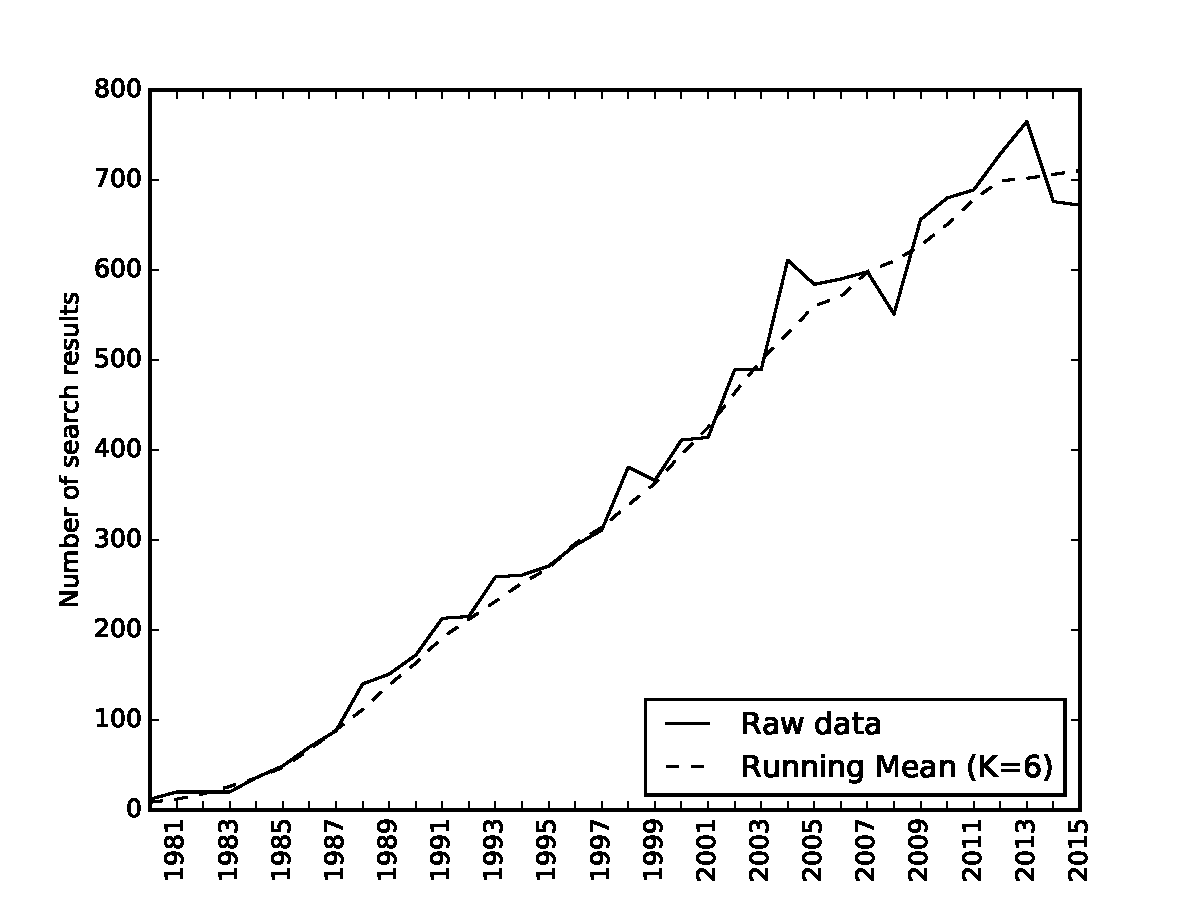
\includegraphics[scale=0.7]{img/cap7-scholar_mig}}
		\caption[Process migration trend in research]{Number of search results in Google Scholar with keyword
		"process migration"}
		\label{fig:cap7-scholar-mig}
\end{figure}


\subsection{Next challenges}
The CRIU project is rapidly evolving thanks to the very active development
community. Since the project is relatively young, it is still unstable,
especially for what concerns the advanced features. In the next years we
expect this project to reach a good level of maturity, such it could be used
also in production environments rather than only in research.

In parallel, new research challenges may arise and old issues may be addressed.
An example of such a case is the possibility managing process migration over
\textbf{heterogeneous processors}. The
explosion of several heterogeneous architectures, from the Graphical Processing
Units to specialized accelerators, requires the adoption of dedicated
techniques
in resource management and application frameworks. Therefore, low-level layer
capable of transparently move processes between processors or nodes with
different
architectures can become an essential feature. Unfortunately, this type of migration is
complex and implementing a working solution requires the involvement of several
computer engineering branches, from operating systems to compilers.
Previous research described in Chapter
\ref{cap:state-of-the-art} provided tools with strong limitations and that work
only for specific scenarios.

The first attempt that can be evaluated for an inclusion in CRIU is the
migration between general purpose architectures with different ISA 
(Instruction Set Architecture), for
instance to migrate a process between \texttt{x86\_64} and \texttt{AArch64}
architectures. The Checkpoint/Restart is already supported by CRIU for both architectures, but migrating processing between them is currently not possible. This because, such a type of migration
requires the translation of all the processors registers, the memory addresses
and other machine-dependent information. Moreover, since there is no one-to-one
correspondence between instructions with different ISA, some sort of
checkpoint barriers must be implemented in the binary code. To understand the
last problem consider the \texttt{MNEG} instruction of \texttt{ARMv8}
(\texttt{AArch64}) having this semantic: \( R_d = -R_n \cdot R_m\). This sort
of specialized instruction does not exist in \texttt{x86\_64} processors and
must be split into a multiplication and a subtraction. Consequently, a
migration mechanism cannot checkpoint the application between multiplication
and subtraction, thus it should consider an atomic operation both of them.
Managing this atomicity for different types of architecture seems not a
straightforward task and it necessarily requires additional support at compiler-level.

The previously described possible improvement in process migration may solve also
the problem of migrating processes between different Linux kernel versions or
different libraries, obviously provided that they expose the same API. As already
described in Chapter \ref{cap:design}, CRIU requires perfectly identical environments.

\subsection{Future developments}
The \texttt{mig} framework is not currently ready for production environments.
A sufficiently stable version has to be developed and possibly integrated
in the mainline repository of Open MPI. The stabilization of the \texttt{mig}
framework and related components requires extensive tests over different
environments and system setups. 

\subsubsection{Iterative Migration}
As we have seen, the transfer time dominates the migration time. This time
becomes an overhead in the overall application execution time, since the
processes
cannot progress during the image migration. However,
CRIU allows the \textbf{Iterative Migration} of processes: the processes
are checkpointed without killing them and, during the processes execution,
the image is transfered. As a result, the execution and image transfer time
are overlapped, this operation is often called \textbf{Pre-Copy}.
Obviously, the transfered image represents the
status of the application at the checkpoint time. Therefore, it does not
represent the current status of the migrating process and it must be updated
with the process memory and the context changes (register, etc.).

In HPC environment, the \emph{iterative migration} shows good performance
results, significantly lowering the migration overhead
\cite{wang2008proactive}. Therefore it can be considered a possible application
improvement to introduce in the \texttt{mig} framework, in order to limit the impact on the wall-time.

\subsubsection{InfiniBand}
The InfiniBand support is the prioritized task to be accomplished in the
development of \texttt{mig} framework. In HPC the InfiniBand networks are
very frequent, because their advantages compared to Ethernet.
InfiniBand presents lower overhead over Ethernet, because the applications are
able to directly communicate with the network adapter without the necessity
of operating system calls. Even considering the
10Gbit and 40Gbit Ethernet, InfiniBand FDR presents higher throughput and
lower latency compared with Ethernet protocols \cite{vienne2012performance}.
Furthermore, in 2014 the new InfiniBand EDR doubles the theoretical throughput
with respect to FDR.

Implementing the InfiniBand support should be a relatively easy task thanks 
to the high modularity of Open MPI. The
functions offered by the TCP \texttt{btl} component have to be replicated in
the InfiniBand \texttt{btl} component. The features provided by other modules -
like \texttt{mig} - are independents from the network protocol used.

\subsubsection{Removing the ORTE daemon granularity}
A further reduction of the \emph{ORTE daemon} overhead could be obtained by moving the
migration granularity to process-level, directly migrating MPI application
processes, instead of the underlying \emph{ORTE daemon}. This requires to change the
active BTL components of the migrating process. Whether \emph{process A} and
\emph{process B} are in the same node communicating via \emph{shared memory}
and
process B migrates towards another node, they have to change the active
\texttt{btl} component to a remote one (e.g. TCP or InfinBand) in order to
resume the connection to the other process. This change requires to address several
synchronization issues.

\subsection{Limitations}

The major limits of the proposed process migration mechanism are in similar
to those of the other C/R based systems: the nodes of HPC systems must be
homogeneous, i.e. the operating system (with kernel version), libraries version
and application binaries must be perfectly identical. Therefore, currently the
\texttt{mig} framework is not exploitable in heterogeneous environments.

Performing the checkpoint with CRIU requires administration
level permissions (\texttt{root} user in Linux) in all the nodes. This
limitation is a partial requirement of CRIU that is in progress to
be dropped by the CRIU development team. However, as previously
described, process migration requires the use of \texttt{unshare} system call,
that in turn requires the \texttt{CAP\_SYS\_ADMIN} capability in Linux. This
permission is usually granted only to the \texttt{root} user. Grant this
permission to non-administrative users may introduce security problems that
should be carefully evaluated and addressed.

In fault tolerant exploitation one of the most important issue to be addressed
is the possibility of migrating also the \emph{ORTE daemon} and
consequently the MPI processes from the HNP. Otherwise, the HNP becomes the
bottleneck in terms of fault-tolerance: the MTTF of the overall system is
reduced to the MTTF of the HNP. Since the \texttt{mpirun} command is actually
an \emph{ORTE daemon}, it would not be difficult to implement the migration of
HNP. We think the only needed change is the adaption of the coordination
protocol between \emph{ORTE daemons} and MPI processes.

\section{Conclusion}

In this thesis we introduced a novel approach to support process migration in
the Open MPI framework. The approach is based on handling the execution of
multiple \emph{ORTE daemon} instances, which can be thought of as the smallest
migratable unit. This is performed transparently to the application and the
non-involved Open MPI frameworks and components.

Compared to other state-of-the-art solutions, one of the major advantages
of our approach is the \emph{maintainability}. The extension introduced in the
Open MPI runtime in fact has a minimal impact on the other Open MPI frameworks.
Furthermore, on the application side the framework does not introduce any
additional API. Therefore its
exploitation it does not require any change on the applications code.

Moreover, the \texttt{mig} framework does not rely on any virtualization layer.
This constitutes a gain in terms of performance with respect to approaches
based
on virtual machine allocation. In this regard, our proposal allows us to
perform
fine-grained migrations, since the resource manager can decide between migrate
an entire application or a subset of its processes. This feature also
increases the controllability of the workload execution.

The integration with Barbeque Run-Time Resource Manager has been implemented
in order to exploit both Open MPI and the \texttt{mig} migration mechanism
in conjunction with a resource manager.
In this regard, a simple policy that solves an
Integer Linear Programming problem has been implemented as a BarbequeRTRM plugin.
This policy 
provides an optimal solution in most cases but it is
usable only with a small number of systems and applications. Therefore,
in the future a greedy policy must be implemented to work with large system,
in particular considering the Exascale computing horizon.

Through experimental tests, we shown how the overhead due to grouping the
application processes on top of several \emph{ORTE daemons} can be considered
negligible.
Conversely, stopping and resuming the processes execution on different nodes,
introduce an overhead dependent on the specific application, its input data
size, the network and the node capabilities.
As a consequence, a resource manager can play a key role to evaluate when a
migration is worth to be performed.

Overall, we can state that the work presented in this thesis is the first
process-level migration feature developed for Open MPI whose control is kept at
system-level (resource manager) and that does not require the code of
applications to be changed.

From the MPI communication standpoint, the lack of \emph{InfiniBand} support is
currently the most important missing feature. However the development of this
component is currently ongoing.

In next years, we can expect an increasing interest in process migration
and in general in C/R techniques. Therefore, the next steps of this work is to
sufficiently debug the code in order to add it to the Open MPI mainline
repository. In this way the \texttt{mig} framework may follow the rapid
developments of Open MPI and CRIU and it can be available for other resource
managers.
